\documentclass[pscyr]{hedwork}
\usepackage[russian]{babel}
\usepackage[utf8]{inputenc}

\usepackage{graphicx}
\graphicspath{{images/}}

\usepackage{color}
\usepackage[colorlinks,linkcolor=black,urlcolor=black]{hyperref}
\renewcommand{\UrlFont}{\rm\small}

\usepackage{setspace}

\newcommand{\pic}[1]{\ref{pic#1}}

\faculty{Факультет электроники и вычислительной техники}
\department{физики}
\subject{дисциплине\\<<Квантовая электроника>>}
\topic{Датчики волнового фронта адаптивных\\оптических систем лазеров}
\student[f]{студентка группы Ф-469\\Слоква В. И.}
\teacher[m]{к. физ.-мат. наук\\Подопригора А. Г.}

\begin{document}
\maketitle
\onehalfspacing

\section{Адаптивные оптические системы}

Примером системы адаптивной оптики может служить система формирования лазерного
пучка для достижения максимальной плотности потока излучения на некотором
объекте. Схема такой системы показана на рис.~\pic{1_1}.

\begin{figure}[ht]
  \center
  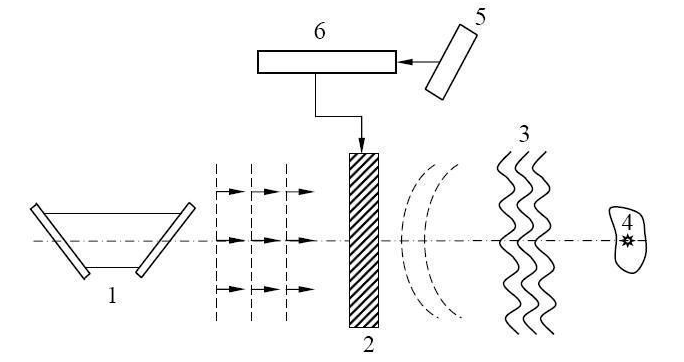
\includegraphics[width=.47\textwidth]{sl_1_1} \hfill
  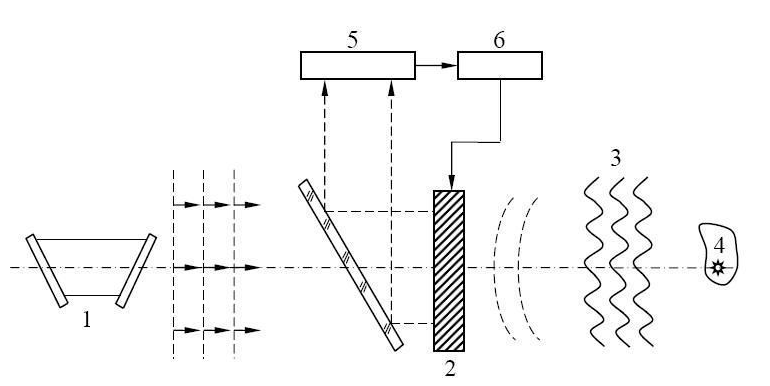
\includegraphics[width=.47\textwidth]{sl_1_2} \\
  \parbox{.47\textwidth}{ \caption{} \label{pic1_1} } \hfill
  \parbox{.47\textwidth}{ \caption{} \label{pic1_2} }
\end{figure}

Корректор~2 преобразует плоский волновой фронт, излучаемый лазером~1, таким
образом, чтобы после прохождения всего оптического пути волновой фронт на
объекте~4 был плоским, плотность потока излучения была максимальной. Для
получения информации об искажении волнового фронта а, следовательно, и для
выработки управляющих сигналов, необходимо время двойного прохождения излучения
от лазера~1 до объекта~4. Расположение датчика~5 перед корректором не означает
размыкания цепи обратной связи, поскольку корректор~2 влияет на характер
освещения объекта~4 и, следовательно, на отраженное им световое поле.

\begin{figure}[ht]
  \center
  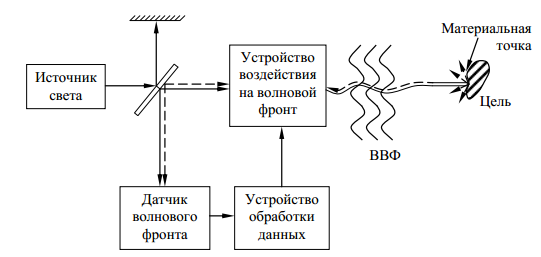
\includegraphics[width=.47\textwidth]{sl_1_3} \hfill
  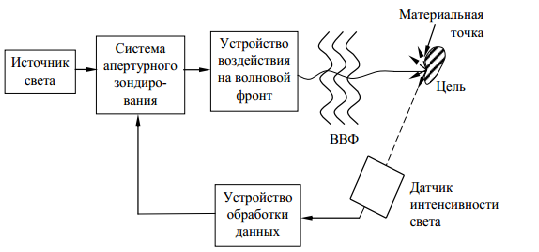
\includegraphics[width=.47\textwidth]{sl_1_4} \\
  \parbox{.47\textwidth}{ \caption{Адаптивная излучающая система, построенная
    на применении метода фазового сопряжения волновых фронтов}
    \label{pic1_3} } \hfill
  \parbox{.47\textwidth}{ \caption{Адаптивная излучающая система, построенная
    на применении принципа повышения резкости изображения}
    \label{pic1_4} }
\end{figure}

Возможно и другое размещение датчика~5, как показано на рис.~\pic{1_2}. В
этом случае отраженное излучение регистрируется после вторичного прохождения
корректора.
 
На рисунке~\pic{1_3} и на рисунке~\pic{1_4} представлены схемы излучающих
систем, предназначенных для создания максимальной плотности потока излучения
(освещенности) на цели. Эти системы работают, как правило, в узком спектральном
диапазоне, используя излучение лазера.

В системе с фазовым сопряжением, схема которой представлена на
рисунке~\pic{1_3}, пучок световых лучей, достигающий цели, отражается от малых
ее участков, которые можно считать материальными точками, образуя сферические
волны. Эти отраженные волны проходят путь распространения в обратном
направлении, и, следовательно, атмосферная турбуленция оказывает на их
пространственные параметры такое же воздействие, как и излучаемый поток световых
лучей. В датчике волнового фронта принимаемая волна сравнивается с волной,
создаваемой в приборе, и устройство обработки данных вычисляет необходимую
коррекцию, которая сопряжена по фазе с измеренным искажением фронта. Затем по
команде устройство  воздействия  на волновой фронт производит требуемую
коррекцию излучаемого волнового фронта. Таким образом, предыскажение, наложенное
на излучаемую волну, компенсирует искажения на пути распространения, благодаря
чему на цель придет волновой фронт сферической формы, которая максимизирует
плотность светового потока на цели. При этом следует иметь ввиду, что суммарное
время двойного прохождения светом турбулентной среды и осуществления коррекции
формы волнового фронта должно иметь меньше или равно времени допустимого
изменения турбулентности.

Вторая изолирующая система, схема которой представлена на рисунке~\pic{1_4},
построена по принципу апертурного зондирования. В этой системе производят
пробные возмущения излучаемого волнового фронта, анализируют световой поток,
вернувшийся от цели, и на основании этого определяют, какие возмущения
увеличивают плотность светового потока. Эти возмущения добавляют в волновой
фронт, и процесс итераций продолжается до тех пор, пока плотность потока не
станет максимальной. 

\section{Датчик волнового фронта}

Датчик волнового фронта (\emph{ДВФ}) является одним из элементов адаптивной
системы корректировки лазерного излучения. Его задача~-- измерять кривизну
волнового фронта и передавать эти измерения на обрабатывающее устройство.

Основными причинами кривизны волнового фронта являются:
\begin{itemize}
  \item турбулентность атмосферы;
  \item неидеальность форм оптических элементов системы;
  \item погрешности при юстировке системы и др.
\end{itemize}

Сегодня существует большое разнообразие ДВФ. Однако, наиболее распространенный
ДВФ строится на основе схемы Шака-Гартмана.

Такой датчик наиболее часто используется в системах корректировки волнового
фронта благодаря своим достоинствам. Одно из главных преимуществ датчика
Шака-Гартмана~-- это его способность измерять большой диапазон наклонов
волнового фронта, когда искажения другими методами (например,
интерференционными) не измерить. Такой датчик может быть использован для
определения аберраций в профиле неколлимированного лазерного пучка. Кроме того,
у него малая чувствительность к механическим вибрациям, и он может работать с
импульсами большой мощности и фемтосекундной длительностью.

\begin{figure}[ht]
  \center
  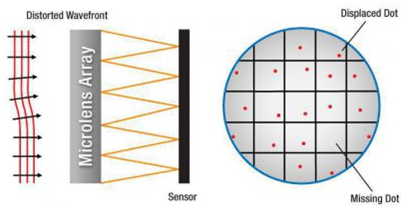
\includegraphics[width=.47\textwidth]{sl_2_1} \hfill
  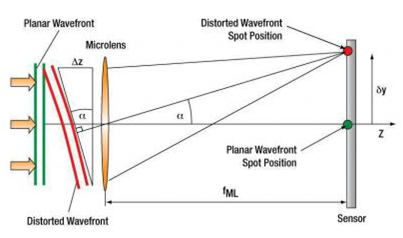
\includegraphics[width=.47\textwidth]{sl_2_2} \\
  \parbox{.47\textwidth}{ \caption{} \label{pic2_1} } \hfill
  \parbox{.47\textwidth}{ \caption{} \label{pic2_2} }
\end{figure}

Принцип работы ДВФ Шака-Гартмана состоит в том, что излучение проходит через
линзовый растр~-- матрицу микролинз (рис.~\pic{2_1})~-- и падает на
фотоприемник. Линзовый растр состоит из идентичных линз, называемых
субапертурой. Они разбивают падающий фронт на малые потоки и фокусируют их на
приемнике, обычно ПЗС-матрице. Когда приходящий волновой фронт плоский, все
сфокусированные изображения расположены в правильной сетке, обусловленной
расположением линз. Если падающая волна имеет какие-либо искажения, то
изображения смещаются со своих номинальных значений. Изображение фокальных пятен
называется гартманограммой. По ее виду можно судить об искривленности волнового
фронта. Более подробно принцип действия можно рассмотреть на рисунке~\pic{2_2}.

Каждая из микролинз массива собирает свет, падающий на его диафрагму и создает
одну точку на плоскости детектора. На рисунке подробно показано прохождение
волнового фронта через одну микролинзу. Сфокусированные на детекторе световые
точки будут располагаться на оси линз (показаны зеленым), только если фронт
плоский. Для волнового фронта с сильными искажениями в области микролинз, место
позиции сместятся в направлении \( X \) и \( Y \) (как показано красной точкой),
так что каждое место находится далеко от оптической оси \( Z \). Угол
\( \alpha \)~-- это угол между искаженным волновым фронтом и плоским волновым
фронтом, как показано на рисунке.

Смещение центров изображений по двум ортогональным направлениям пропорционально
средним наклонам волнового фронта в этих направлениях по субапертурам. Таким
образом, ДВФ Шака-Гартмана измеряет наклоны волнового фронта, сам фронт
восстанавливается из массива наклонов. Наклоны оцениваются из смещений
центроидов изображений фокальных пятен:
\[
  x = \frac{\sum\limits_{ij} x_{ij} I_{ij}}{\sum\limits_{ij} I_{ij}}, \qquad
    y = \frac{\sum\limits_{ij} y_{ij} I_{ij}}{\sum\limits_{ij} I_{ij}}
\]
где \( I_{ij} \)~-- интенсивность в фокальном пятне, \( x_{ij} \)~-- положение
фокального пятна по оси \( x \), \( y_{ij} \)~-- положение фокального пятна по
оси \( y \).

У датчика Шака-Гартмана есть четыре параметра, которые влияют на его разрешающую
способность. Это количество микролинз, которые охватывает активную область
детектора, диапазон и чувствительность измерений, а также фокусное расстояние
микролинз.
 
Количество микролинз показывает, какое максимальное количество коэффициентов
Цернике необходимо рассчитать для алгоритма восстановления. Эти коэффициенты
показывают величину тех или иных аберраций. При выборе количества линз нужно
учесть степень искажения сигнала, т.~е. сколько коэффициентов необходимо для
эффективного представления истинной аберрации волнового фронта.

Чувствительность \( \alpha_{\min} \)~-- это функция минимального смещения пятна,
которое может быть обнаружено, приближенно она описывается следующим уравнением:
\[
  \alpha_{\min} = \delta y_{\min} / f,
\]
где \( f \)~-- фокусное расстояние микролинзы.
 
Динамический диапазон определяется максимальным смещением, которое можно
измерить:
\[
  \alpha_{\max} = \delta y_{\max} / f = D / 2f,
\]
где D~-- диаметр микролинзы.

Эти уравнения были получены при использовании приближения малых углов.
Минимальное перемещение \( \delta y_{\min} \) зависит от размера пикселя
детектора, точности используемого алгоритма, а также от соотношения сигнал/шум
датчика.
 
Еще одно достоинство ДВФ Шака-Гартмана~-- это его ахроматичность, т.~е. наклоны
волнового фронта не зависят от длины волны излучения.

В настоящее время для некоторых систем требуются компоненты с минимальными
габаритами и простыми схемами исполнения. Для таких систем изготавливают ДВФ с
клиновым растром, т.~е. линзы заменяются оптическими клиньями. Углы при вершине
определяются, исходя из заданной координаты центра зоны контроля на
чувствительной площадке приемника. Необходимое количество клиньев меньше, чем
количество микролинз. Такие датчики используются для выравнивания распределения
света по поперечному сечению пучка. Также используют матрицы, состоящие из
макролинз. Разрешающая способность таких датчиков гораздо хуже, но стоимость и
габариты существенно уменьшаются.

\pagebreak % -------------------------------------------------------------------
\renewcommand{\bibname}{Список литературы}

\begin{thebibliography}{9}
  \bibitem{1} Беспалов, В.~И., Пасманик, В.~А. Нелинейная оптика и адаптивные
    лазерные системы~/ В. И. Беспалов, В. А. Пасманик.~-- М.: Наука,~1986.~--
    136~с.
  \bibitem{2} Датчики волнового фронта. Режим доступа:
    \url{http://laser-portal.ru/content_706}\\
    (дата обращения 07.12.2013).
  \bibitem{3} Берченко, Е.~А., Калинин, Ю.~А., Киселев, В.~Ю., Полынкин, М.~А.,
    Прилепский, Б.~В., Филатов, А.~С. Датчики волнового фронта~//
    Лазерно-оптические системы и технологии, ФГУП "НПО АСТРОФИЗИКА"~--
    М.,~2009.~-- С.~64--69. 
  \bibitem{4} Ермолаева, Е.~В., Зверев, В.~А., Филатов, А.~А. Адаптивная
    оптика~/\\ Е.~В. Ермолаева, В.~А. Зверев, А.~А. Филатов~-- СПб.: НИУ
    ИТМО,~2012.~-- 297~с.
\end{thebibliography}

\end{document}